\chapter{Ideen und Konzepte}
TODO einleitung

% Hier geht es um die Fragestellung, wie Sie die formulierten Ziele der Arbeit erreichen wollen.
% Sie halten z.B. erste, grobe Ideen, skizzenhafte Lösungsansätze fest. Gibt es mehrere Wege, Ansätze
% um dieses Ziel zu erreichen, begründen Sie hier, warum Sie einen bestimmten Weg einschlagen.
% Beispiel für ein Softwareprojekt: Erste Gedanken über eine grobe Systemarchitektur. Ist z.B. eine
% Microservice-Architektur angebracht? Welche Alternativen bestehen, wo gibt es Problempunkte? Die
% Umsetzung, die Beurteilung der Machbarkeit und die detaillierte Beschreibung der umgesetzten
% Architektur sind dann Teil der Realisierung.
% Abgrenzung zu Kapitel 5:
% - Besteht ein wesentliches Projektziel darin, für Ihre Kunden z.B. ein Security-Konzept, ein
% Kommunikations-Konzeptes, ein IT-Fachkonzept oder ein anderes Fach-Konzept zu erstellen, dann
% wird die Entwicklung dieser (fachlichen) Konzepte unter «Realisierung» beschrieben (sie sind ja der
% eigentliche Kern Ihrer Arbeit).
% - Besteht z.B. ein wesentliches Ziel der Arbeit darin, eine passende Software-Architektur zu
% evaluieren, dann gehören die entsprechenden Beschreibungen ins Kapitel 5.


% \section{Konfiguration} \label{idea_config} %todo delete
% \subsection{Motivation}
% Bei der Landis+Gyr werden verschiedenen Stromzählermodelle entwickelt. Der DlmsQuickAccess soll mit möglichst allen kommunizieren können.
% Wie bereits in XY TODO erwähnt, wird für die Kommunikation Code der ATS verwendet.
% Damit dieser richtig funktionieren kann, werden folgende zwei Dateien benötigt:
% - AddressList
% - DLMS.xml
% Für die Auflistung aller Objekte eines Zählers wird zusätzlich ein ObjectModel als XML Datei benötigt.
% Diese drei Dateien unterscheiden sich von Produkt zu Produkt. Ebenfalls muss berücksichtigt werden, dass sich die Informationen in diesen Dateien jederzeit ändern können.
% Insbesondere beim ObjectModel ist dies regelmässig der Fall.

% Diese Konfigurationen sollen somit von den Produktteams verwaltet und versioniert werden können.

% \subsection{Lösungsidee}
% Eine Konfigurationsdatei in welcher die zuvor erwähnten Dateien definiert sind. Die soll im YAML format geschrieben sein, was das Bearbeiten vereinfacht.
% Jedes Produktteam kann diese Konfigurationsdatei im Repository des Produktquellcodes ablegen und versionieren.

% TODO
% damit sich der DlmsQuickAccess beim Betriebssystem so registrieren kann, dass 
% Diese Konfiurationsdateien sollen die Endung \".dlmsquickaccess\" tragen, 

% Um das Wechseln zwischen Produkten zu vereinfachen, soll sich der DlmsQuickAccess zuvor verwendete Konfigurationen merken, so dass der Benutzer diese auswählen kann.


% TODO ufschribe, was passiert bim erste start und bi doppelclick.


\section{Aufbau Benutzerschnittstelle}\label{aufbauUI}
Die Benutzerschnittstelle soll in zwei Bereiche aufgeteilt werde.
\begin{figure}[H]
   \centering
   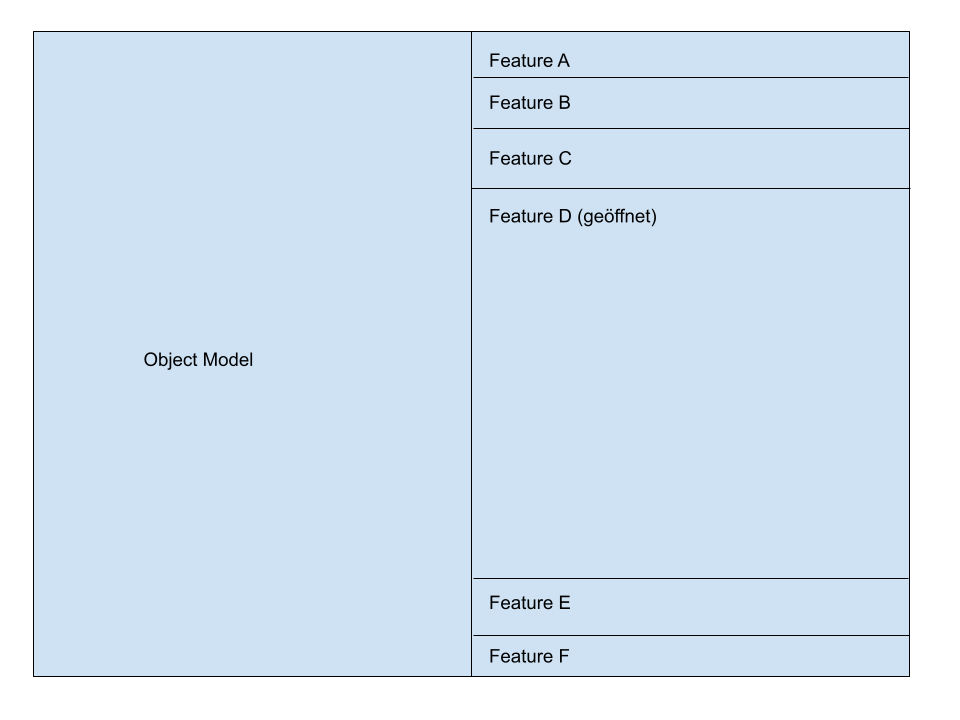
\includegraphics[width=1.0\textwidth]{gfx/App strucutre sketch.png}
   \caption{
      Sketch des Aufbau der Benutzeroberfläche
      }
      \label{fig:uisketch}
   \end{figure}
Der erste Bereich soll Object Model beinhalten.
Im folgenden Abschnitt wird darauf detailliert eingegangen.
Dieser Bereich soll alle Grundfunktionen der Applikation abdecken.
Also jene, welche bei der zu ersetzenden Applikation, dem \ac{DMT2} vorhanden sind.
Der zweite Bereich soll Platz für die erweiterten Funktionen bieten.
Die Idee ist, dass diese vertikal übereinander aufgelistet sind.
Möchte der Nutzer eine Funktion verwenden, so kann er diese anklicken und entsprechenden Controls erscheinen in der Liste.
In Abbildung \ref{fig:uisketch} ist gezeigt, wie die beiden Bereiche horizontal nebeneinander angezeigt werden sollen.
Auf der rechten Seite ist zu erkennen, wie die verschiedenen Features übereinander aufgelistet werden sollen.
\textit{Feature D} nimmt dabei mehr Platz ein als die anderen.
Damit wird dargestellt, dass dieses von Nutzer angewählt und geöffnet wurde.
Eine dieser Funktionen sind die Favoriten.
Wie deren Benutzerschnittstelle aussehen soll, ist im Abschnitt \ref{uifavorites} aufgeführt.

\subsection{Object Model}
Der \textit{Quick Access} des \ac{DMT2} besteht aus vier Teilen.
In Abbildung \ref{fig:dmt2QuickAccess} ist dies dargestellt.
Oben links sind alle Objekte angezeigt.
Rechts daneben werden die Attribute und Methoden des aktuell aktiven Objekts angezeigt.
Fürs Lesen und Schreiben werden in den unteren beiden Teilen des Fensters jeweils der Request und die Response in einer als \text{XML} Text dargestellt.

\begin{figure}
   \centering
   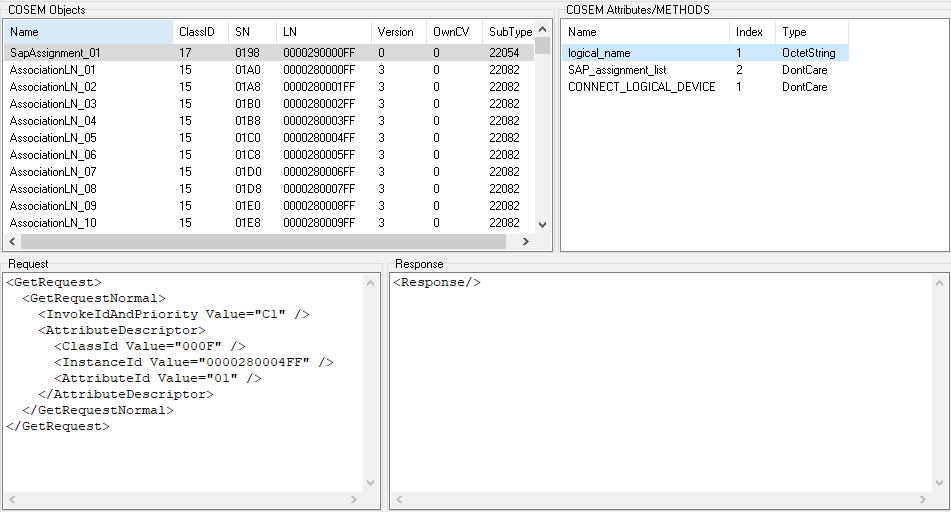
\includegraphics[width=1.0\textwidth]{gfx/UI_DMT2.png}
   \caption{
      Quick Access Fenster des \ac{DMT2}
      }
      \label{fig:dmt2QuickAccess}
\end{figure}
In der neuen Anwendungen sollen diese viert Teile in einer einzelnen Komponente kombiniert dargestellt werden.
Wie dies aussehen kann, ist in Abbildung \ref{fig:objectModelUIsktech} gezeigt.
Die Objekte, beispielsweise \textit{Profile 1}, werden untereinander aufgelistete.
Wird ein Objekt angeklick, soll vergrössert sich dieses und die Attribute und Methoden werden ersichtlich.
Wird ein Attribute gelesen, so soll der Wert in einem Textfeld neben dem Attribut dargestellt werden.
Das bietet den Vorteil, dass die Werte mehrere ausgelesener Attribute gleichzeitig angeschaut werden können. 
Dies ist beim \textit{Quick Access} nicht möglich, da der Bereich mit der Response bei jedem Auslesen überschrieben wird.
Die Textfelder, welche für das Anzeigen der gelesenen Werte verwendet werden, sollen jeweils auch für das Schreiben von Werten verwendet werden.

\begin{figure}
   \centering
   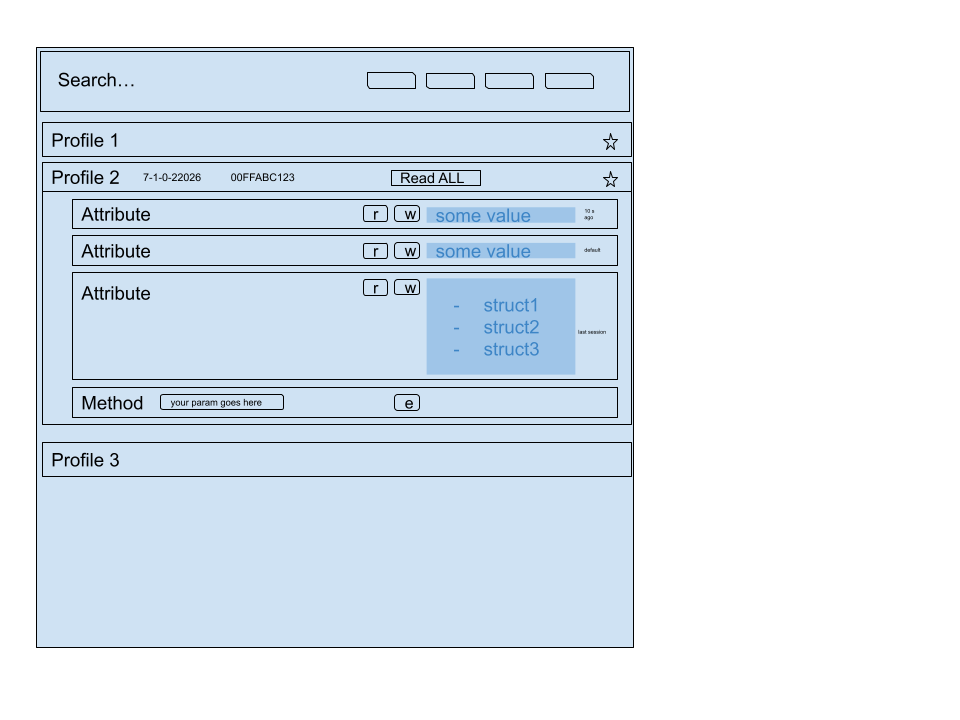
\includegraphics[width=1.0\textwidth]{gfx/Object Explorer Sketch.png}
   \caption{
      Sketch der Object Model Komponente
      }
      \label{fig:objectModelUIsktech}
\end{figure}


\subsection{Suchen und filtern}\label{searchandfilterUiSktech}
Im Sketch zum Object Model (Abbildung \ref{fig:objectModelUIsktech}) ist der Bereich oberhalb der Objekte für die Such- und Filterkomponente vorgesehen.
Eine Idee zur Umsetzung dieser ist in Abbildung \ref{fig:searchFilterSketch}.
Um die Objekte nach ClassId zu filtern, können die Textfelder im oberen Bereich des Sketchs verwendet werden.
Das Textfeld im unteren Bereich ist für die textbasierte suche gedacht.
Ein Schalter in der Mitte soll dazu da sein, dass bei der Textsuche zwischen Objekten und Attributen rsp. Methoden gewechselt werden kan.
Der \textit{Find} Knopf soll die Parameter anwenden, mit dem \textit{Reset} Knopf sollen diese zurückgesetzt werden.

\begin{figure}
   \centering
   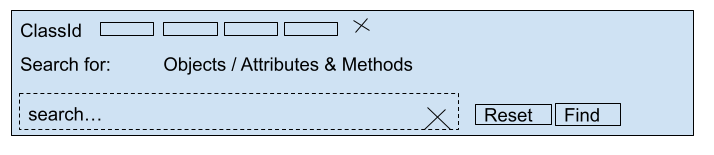
\includegraphics[width=1.0\textwidth]{gfx/Search _ Filter sketch.png}
   \caption{
      Sketch der Komponente fürs Suchen und Filtern des Object Models
      }
      \label{fig:searchFilterSketch}
\end{figure}

\subsection{Favoriten}\label{uifavorites}
In einem vorherigen Abschnitt wurde erklärt, dass auf die rechte Hälfte der Benutzerschnittstelle Platz für unterschiedliche Features haben soll.
Dort sollen auch die Favoriten aufgelistete werden.
Diese sollen in zwei Bereichen dargestellt werden und nehmen somit auch zwei Plätze in der Features Liste ein.
Einer für favorisierte Objekte und einer für favorisierte Attribute und Methoden.
In Abbildung \ref{fig:favoritesSketch} ist ersichtlich, wie Attribute und Methoden gruppiert dargestellt werden sollen.

\begin{figure}
   \centering
   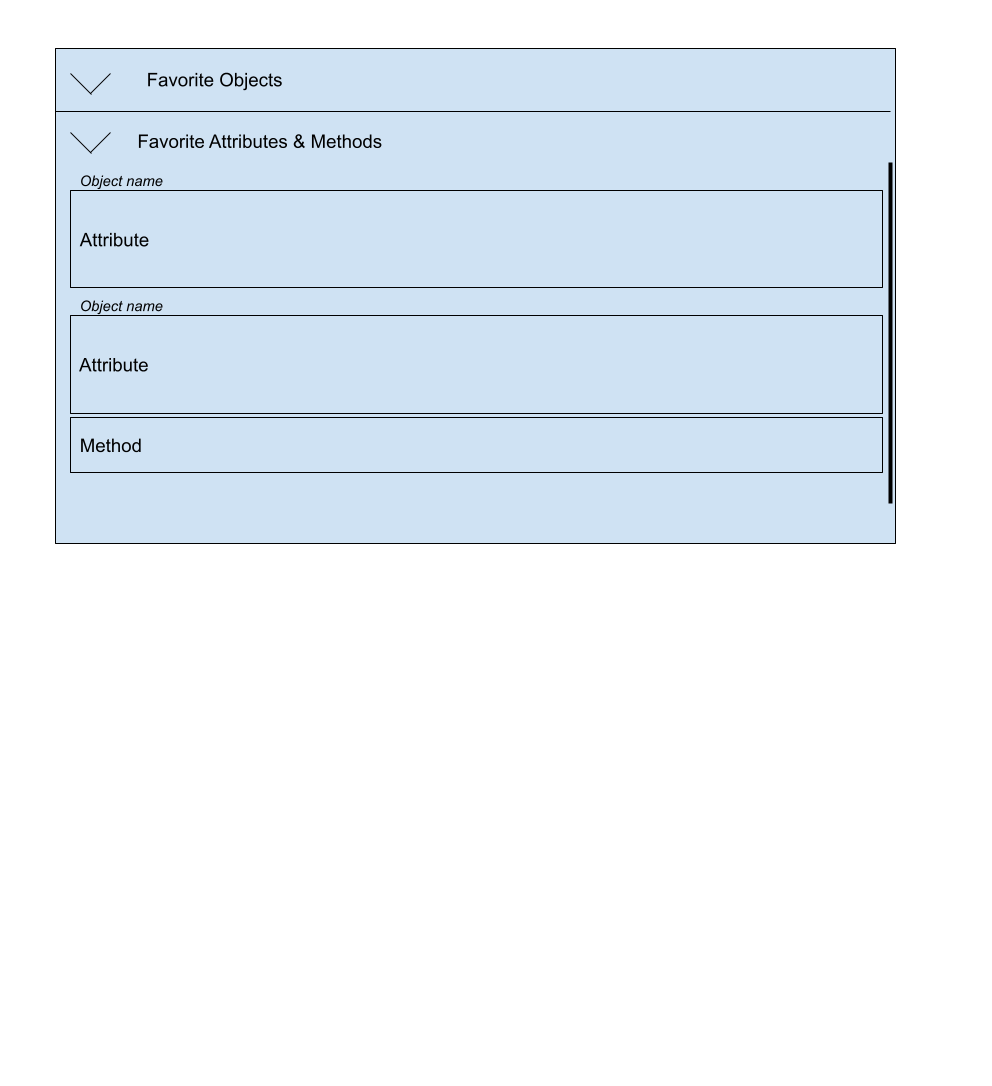
\includegraphics[width=1.0\textwidth]{gfx/Favorites Sketch.png}
   \caption{
      Sketch der Favoriten Komponente
      }
      \label{fig:favoritesSketch}
\end{figure}

\pagebreak
\section{Testkonzept}
Um sicherstellen, dass die Applikation und deren Komponenten richtig funktionieren, wurden verschieden Arten von Tests eingesetzt.
Die unterscheiden sich primär im Umfang des Getesteten. 
In den folgenden Abschnitten werden sie detailliert beschrieben und verglichen.

\subsection{Unittests}
Unittests werden so eingesetzt, dass sie die Funktionalität einer einzelnen Klasse testen.
Abhängigkeiten zu anderen Klassen sollen jeweils durch Mocks ersetzt werden.
Die Tests werden jeweils parallel zum getesteten Code geschrieben.
Mehr dazu im Abschnitt \ref{tdd} Test Driven Development.
Um sicherzustellen, dass zuvor implementierte Funktionen nicht durch neue Änderungen nicht zerstört werden, werden alle Unittest regelmässig und automatisiert ausgeführt.
Dies wurde mit der CI/CD Pipeline realisiert. Diese ist im Abschnitt TODO detailliert beschrieben.

\subsection{Modultests}
Bei den Modultests wird das Zusammenspiel mehrere Klassen getestet, welche gemeinsam ein Modul bilden.
Dabei soll nur das öffentliche Interface des Moduls verwendet werden.
Abhängigkeit, welche nicht Teil dieses Moduls sind, werden wie bei den Unittests durch Mocks oder Fakes ersetzt.
Im Gegensatz zu den Unittests ist der Zeitpunkt für das Schreiben der Modultests nicht definiert.
Sie sollen so eingesetzt werden, wie sie für den Entwicklungsprozess hilfreich sind.

Beispiel: Mittels Refactoring soll das interne Design eines bestehenden Moduls verbessert werden.
Um sicherzustellen, dass das Modul nach dem Refactoring noch korrekt funktioniert, werden zuvor Modultests geschrieben, welche die öffentliche Schnittstelle des Moduls testet.
Da sich diese beim Refactoring nicht verändert, können die Modultests auch noch nach dem Refactoring ausgeführt werden.
Unittests, welche interne Klassen getestet haben sind womöglich nicht mehr brauchbar, da sich die internen Schnittstellen bei Refactoring stark verändert haben.

Im Bezug auf die regelmässige und automatisierte Ausführung sollen sich Modultests nicht von Unittests unterscheiden.


\subsection{Integrationstests}\label{Integrationstests}
Integrationstests sind im dazu da, die Funktionalität von Komponenten sowie das Zusammenspiel dieser mit anderen zu Testen \parencite{winter2012integrationstest}.
Im Gegensatz zu Unit- und Modultests wird auf den Einsatz von Mocks oder Fakes verzichtet um ein möglichst realitätsnahen Testaufbau zu erreichen.
Da die Kommunikation mit Stromzähler für die zu testende Applikation zentral ist, wird für das Ausführen der Integrationstests ein angeschlossener Stromzähler benötigt.
Im Rahmen dieses Projekts war es nicht mögliche einen Testagent mit angeschlossenem Zähler bereit zu stellen.
Deshalb wurden die Integrationstests ausschliesslich lokal auf dem Rechner des Entwicklers ausgeführt.


\section{Model-View-ViewModel}\label{mvvm}
\ac{MVVM} ist ein Entwurfsmuster welches 2005 von Microsoft vorgestellt wurde.
Sein Ziel ist es, das Daten, Logik und Views einer Anwendung unabhängig von einander entwickelt und getestet werden können.
Es besteht aus folgenden Sichten:
\begin{itemize}
   \item Model: Das Domänen Model der Applikation
   \item View: XAML Komponenten, welche die visuellen Aspekte der Applikation definieren
   \item ViewModel: Klassen bestehend aus Properties und Commands, welche von den Views verwendet verden
\end{itemize}

% TODO Image source : https://www.dev-insider.de/was-bedeutet-mvvm-a-1103448/
\begin{figure}[H]
   \centering
   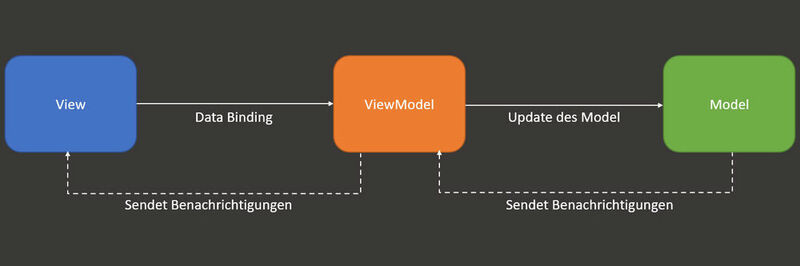
\includegraphics[width=1.0\textwidth]{gfx/mvvm.jpg}
   \caption{
      Das Model-View-ViewModel Entwurfsmuster
   }
   \label{fig:mvvm}
\end{figure}
Die ViewModels sind dabei der wichtigste Teil, da sie den Zustand der Applikation abbilden.
Sie sammeln die für die Views benötigten Daten zusammen und stellen sie als Properties bereit.
Mittels DataBinding referenzieren die Views diese Properties, ohne dabei das konkrete ViewModel kennen zu müssen \parencite{vermeir2022desktop}.
Wie \ac{MVVM} für diese Arbeit umgesetzt werden kann, ist im folgenden Abschnitt beschrieben.




\section{Architektur}
% TODO, evtl verschieben zu Realisierung und hier nur die grundlegenden Idee aufzeigen. Wie MVVM angewendet wurde
Der Quellcode der Anwendung ist in mehrere C\# Projekte aufgeteilt.

Dies soll die Wiederverwendbarkeit der Komponenten sicherstellen.
Wenn in Zukunft eine Komponente wie bspw. die Kommunikation ausgetauscht werden soll, so müssen nur in einem spezifischen Teil des Codes Änderungen vorgenommen werden.

\begin{figure}[H]
   \centering
   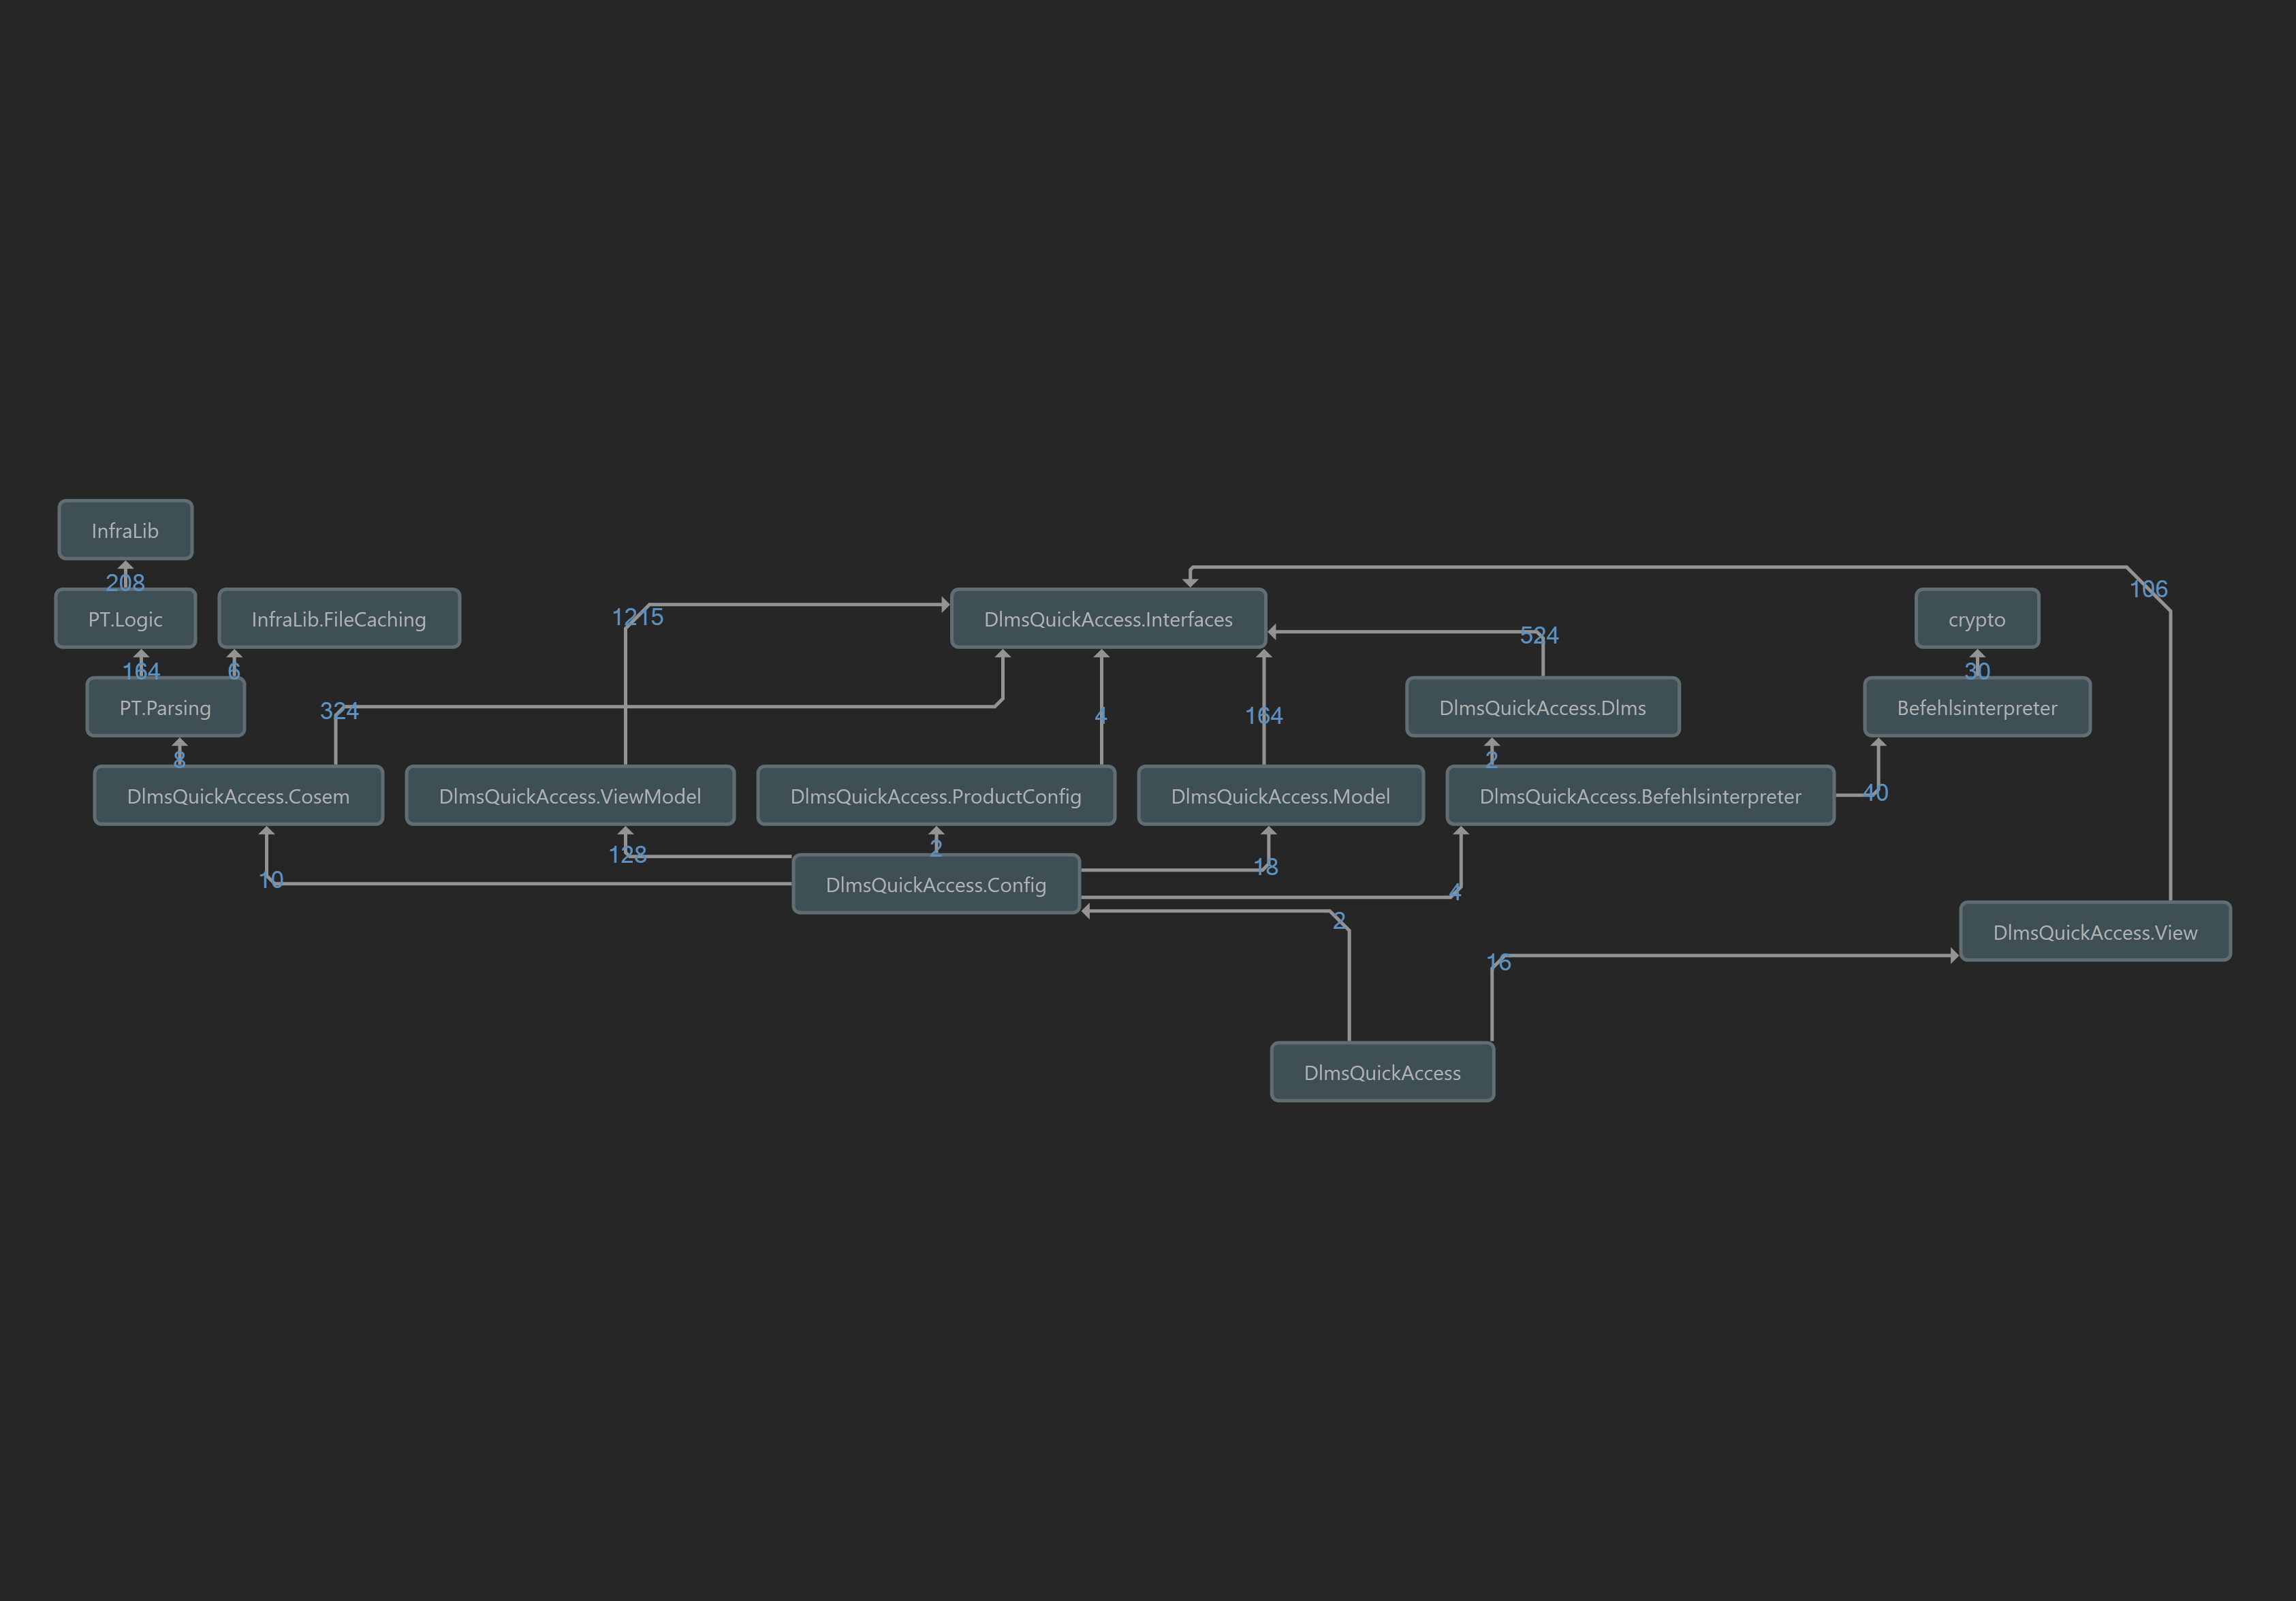
\includegraphics[width=1.0\textwidth]{gfx/Architecture view for DlmsQuickAccess.png}
   \caption{
      Abhänigkeiten der Projekte
   }
   \label{fig:projectDependencies}
\end{figure}

In der Abbildung \ref{fig:projectDependencies} sind alle\footnote{Die Testprojekte wurde einfachheitshalber weggelassen.} Projekte und deren Abhängigkeit aufgezeigt.
Diese werden in den folgenden Abschnitten näher beschrieben.

\subsection{DlmsQuickAccess}
Dieses Projekt ist der Einstiegspunk der Anwendung.
Die Klasse \textit{App} lässt sich mit der \texttt{main()} Method vergleichen, welchen den meisten C basierten Sprachen als erstes ausgeführt, wenn ein Programm gestartet wird.
Diese lädt \textit{Windows} und \textit{Controls} aus dem DlmsQuickAccess.View Projekt und zeigt diese dem Nutzer an.



\subsection{DlmsQuickAccess.View}
Sämtliche Komponenten der Benutzerschnittstelle, also \textit{Windows} und \textit{Controls}, sind in diesem Projekt definiert. 
Nebst der Abhängigkeit zum Framework WinUI3, welches für die Darstellung der Element der Benutzerschnittstelle benötigt wird, gibt es nur eine einzige Abhängigkeit, jene zu DlmsQuickAccess.Interfaces.
Diese ist dazu da, dass die Controls die Interfaces der ViewModels kennen, auf welche sie binden.
Das Zusammenspiel von View und ViewModel ist im Abschnitt \ref{mvvm} beschrieben.
Währen diese Interfaces im selben Projekt wie die Controls definiert, so hätten die Implementationen der ViewModels eine Abhängigkeit auf DlmsQuickAccess.View.
Um eine solche Koppelung zu vermeiden, wurden die Interfaces in ein eigenes Projekt ausgelagert.


\subsection{DlmsQuickAccess.ViewModel}
Die zuvor erwähnten ViewModel Interfaces sind in diesem Projekt implementiert.
Nebst den eigentlichen ViewModel Klassen enthält das Projekt mehrere Factory Klassen, welche für die Instanziierung der ViewModel Klassen zuständig sind.
Hier wurde das Factory Method Erstellungsmuster angewendet \parencite{designPatterns}.
In Abbildung \ref{fig:filterViewModel} ist die \textit{FilterViewModelFactory} Klasse zur Erstellung des \textit{FilterViewModel} aufgezeigt.
\begin{figure}[H]
   \centering
   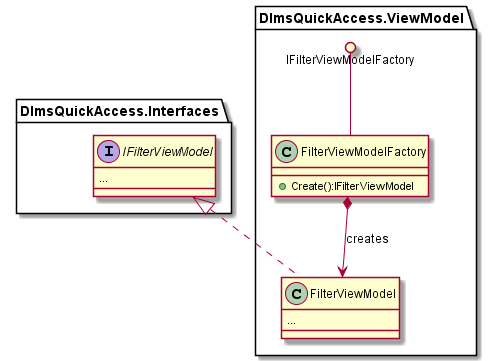
\includegraphics[width=0.7\textwidth]{gfx/Filter ViewModel.png}
   \caption{
      Unvollständiges Klassendiagramm zum FilterViewModel und FilterViewModelFactory
      }
      \label{fig:filterViewModel}
\end{figure}

Dieses Design vereinfacht das Testen der Instanziierungen.
Ein weitere Vorteil ist, dass eine Factory eine andere Factory mittels Assoziation verwenden kann, deren konkrete Implementation jedoch nicht kennen muss.
In Abbildung \ref{fig:vmfactories} ist ganz oben die \textit{MainWindowViewModelFactory} Klasse abgebildet, welche für die Erstellung des \textit{MainWindowViewModel} zuständig ist.
Dieses ViewModel beinhaltete alle anderen ViewModels welche für die verschiedenen Bereiche der Applikation benötigt werden.
Um diese zu erstellen verwendete \textit{MainWindowViewModelFactory} Instanzen der \textit{IObjectModelViewModelFactory} und \textit{IFavoritesViewModelFactory} welche selbst weitere Factories verwenden.
Das bringt den Vorteil, dass die einzelnen Factory Klassen nicht aneinander gekoppelt sind.
Sie werden erst bei ihrer Instanziierung mittels Dependency Injection miteinander verbunden.
Diese ist Teils des Projekts DlmsQuickAccess.Config (\ref{dqa:config}).
   
\begin{figure}[H]
   \centering
   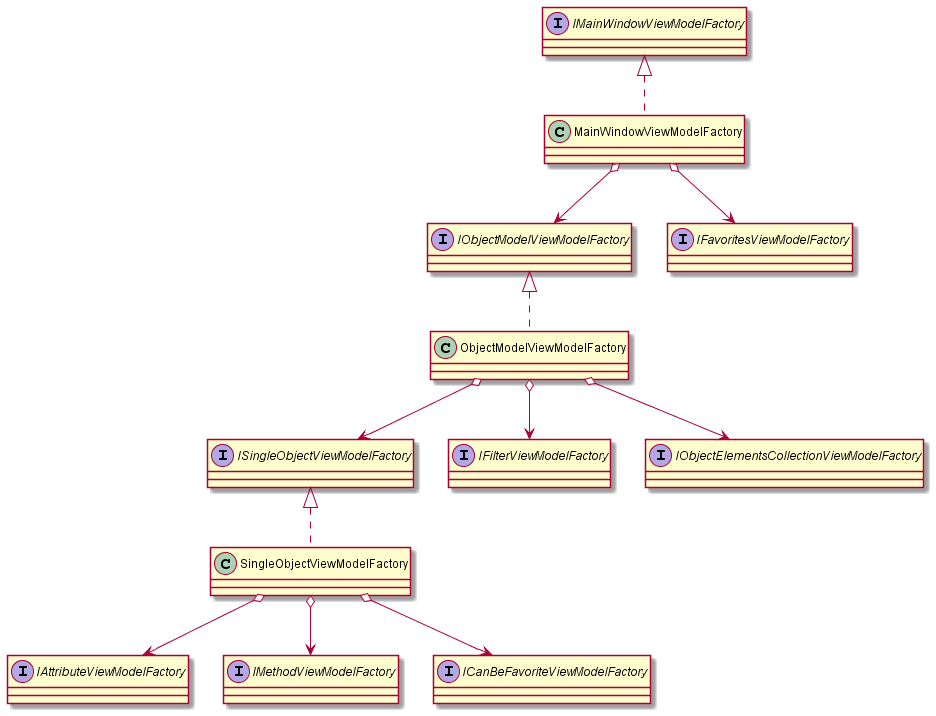
\includegraphics[width=1.0\textwidth]{gfx/vmfactories.png}
   \caption{
      Unvollständiges Klassendiagramm zu den verschiedenen ViewModel Factories.
      }
   \label{fig:vmfactories}
\end{figure}

\subsection{DlmsQuickAccess.Model}


\subsection{DlmsQuickAccess.Config}\label{dqa:config}

\subsection{DlmsQuickAccess.Interfaces}

\subsection{DlmsQuickAccess.ProductConfig}
External dependency to yamllib


\subsection{DlmsQuickAccess.Dlms}
evtl widerverwendbar

\subsection{DlmsQuickAccess.Cosem}
evtl widerverwendbar
infralib etc.

\subsection{DlmsQuickAccess.Befehlsinterpreter}
isolation des Befehlsinterpreter

